{}\documentclass[letterpaper,
compress,
xcolor=x11names,
%draft,
]{beamer}
% Package imports
\usepackage{mathtools} % imports `amsmath'
\DeclareMathOperator{\sech}{sech}
\usepackage{amssymb}
\usepackage{fixltx2e}
\usepackage{lmodern}
\usepackage{movie15}
%\usepackage{media9}
\usepackage{microtype}
\usepackage{animate}
\usepackage{subcaption}
\captionsetup{compatibility=false}

% I just did this
\usepackage[english]{babel}
\usepackage[utf8]{inputenc}
\usepackage{amsmath}
\usepackage{graphicx}
\usepackage[colorinlistoftodos]{todonotes}
\usepackage{tikz}
\usetikzlibrary{tikzmark}
\usepackage{array}
\usepackage{layout}
\usepackage{multicol}
\usepackage{multirow}
\usepackage{booktabs}
%I just did this

% `beamer' configuration
\usefonttheme{professionalfonts}
\useoutertheme[subsection=false,]{miniframes}
\setbeamercolor*{alerted text}{fg=red}
\setbeamercolor*{example text}{fg=black}
\definecolor{CSU_green}{RGB}{30, 70, 43}
\definecolor{CSU_gold}{RGB}{200, 195, 114}
\setbeamercolor*{lower separation line head}{bg=CSU_gold}
\setbeamercolor*{section in head/foot}{fg=white,bg=CSU_green}
\setbeamercolor*{subsection in head/foot}{bg=white}
\setbeamercolor*{upper separation line head}{bg=CSU_gold}
\setbeamercolor*{page number in head/foot}{fg=CSU_green}
\setbeamercolor*{normal text}{fg=black,bg=white}
\setbeamercolor*{palette tertiary}{fg=black,bg=black!10}
\setbeamercolor*{palette quaternary}{fg=black,bg=black!10}
\setbeamercolor*{structure}{fg=black}
\setbeamerfont{frametitle}{shape=\scshape}
\setbeamerfont{institute}{shape=\scshape}
\setbeamerfont{section in head/foot}{shape=\scshape}
\setbeamerfont{subsection in head/foot}{shape=\scshape}
\setbeamertemplate{bibliography item}{}
\setbeamertemplate{itemize items}[ball]
\setbeamertemplate{navigation symbols}{}
\setbeamertemplate{footline}[frame number]
\usetikzlibrary{calc,arrows}
\graphicspath{{graphics/}{graphics/movies/}{graphics/images/}}
\usepackage{remreset}                  % hack to display beamer navigation
\makeatletter                          % circles even if not declaring
\@removefromreset{subsection}{section} % subsections
\makeatother                           % see: http://tex.stackexchange.com/a/2078
\setcounter{subsection}{1}             % see: https://bitbucket.org/rivanvx/beamer/issue/218

% `biblatex' configuration
\usepackage[backend=biber,
style=authortitle-comp,
]{biblatex}
\addbibresource{presentation.bib}

% `enumitem' configuration
\usepackage{enumitem}
\setlist[itemize,1]{label=\usebeamertemplate{itemize item}}
\setlist[itemize,2]{label=\usebeamertemplate{itemize subitem}}
\setlist[itemize,3]{label=\usebeamertemplate{itemize subsubitem}}
\DeclareMathOperator{\sinc}{sinc}


% `graphicx' configuration
\usepackage{graphicx}
\begin{document}
	\title{Interpolation}
	%\subtitle{MATH-151:  Mathematical Algorithms in Matlab}
	\author{MATH-151:  Mathematical Algorithms in Matlab}
	\date[202X]{September 18, 2023}
	\titlegraphic{
\includegraphics[height = 3cm]{CSU_Ram_Logo.jpg}}



%%%%%%%%%%%%%%%%%%%%%%%%%%%%%%%%%%%%%%%%%%%%%%%%%%%%%%

\begin{frame}
\titlepage
\end{frame}
%%%%%%%%%%%%%%%%%%%%%%%%%%%%%%%%%%%%%%%%%%%%%%%%%%%%%%%%%
\section{Interpolation}

\begin{frame}{Fitting the Data}
	\footnotesize
	\begin{itemize}
		\item Sometimes we are given some information and want to find a function that agrees with the data. This is a process called \textbf{interpolation}
		\begin{itemize}
			\item Some of you have probably seen least-squares fits or regression before, that seeks to match the ``trend" of the data, however with interpolation, we want to describe the functional relationship of the data \textbf{and} make sure all of our data points are included
			\begin{center}
				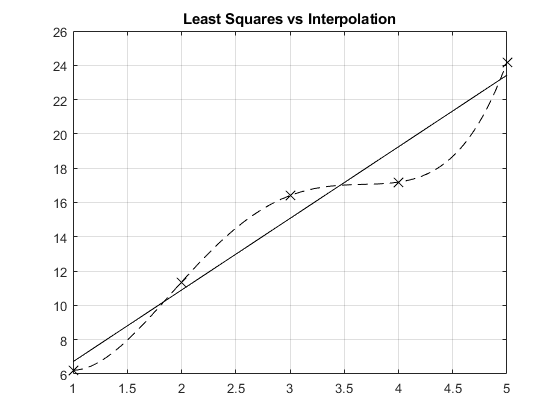
\includegraphics[height = 3cm]{interp_vs_ls.png}
			\end{center}
		\end{itemize}
		\item Most often we use polynomials as our \textbf{interpolants}, but different sets of functions can also be used!
	\end{itemize}
\end{frame}

%%%%%%%%%%%%%%%%%%%%%%%%%%%%%%%%%%%%%%%%%%%%%%%%%%%%%%%%%

\begin{frame}{When is Interpolation Used?}
	\footnotesize
	\begin{itemize}
		\item Interpolation is useful in many purposes when we are interested in representing data with a smooth function that captures changes in slope. For example
		\begin{itemize}
			\item Plotting a smooth curve through data
			\item Reading between entries of a data table
			\item Differentiation or integration of function data
			\item Approximating a complicated function with a simpler one
			\item Using trigonometric functions to interpolate uniformly-spaced data points is called the Discrete Fourier Transform (or DFT) and commonly used in signal processing.
		\end{itemize}
	\end{itemize}
\end{frame}

%%%%%%%%%%%%%%%%%%%%%%%%%%%%%%%%%%%%%%%%%%%%%%%%%%%%%%%%%
\section{Polynomial Methods}

\begin{frame}{Lagrange Method}
	\footnotesize
	\begin{itemize}
		\item Lagrange's method is centered around creating terms that equal $f(x_i)$ when $x=x_i$ and 0 when $x=x_j, j\neq i$.
		\item Let's start with the second part, how do we make our term be 0, when our $x$ is any of our other points? We multiply by $(x-x_j)$ for all the $j\neq i$ 
		\begin{center}
			We write this $\displaystyle\prod_{j=1, j\neq i}^{N}(x-x_j)$
		\end{center}
		\item How do we make it correct when $x=x_i$? We take our product above and divide by $(x_i-x_j)$ for each $j\neq i$ so we get 1, then multiply by $f(x_i)$
		\begin{center}
			This gives us  $\displaystyle f(x_i)\frac{\prod_{j=1, j\neq i}^{N}(x-x_j)}{\prod_{j=1, j\neq i}^{N}(x_i-x_j)}$
		\end{center}
		\item We repeat this for each of our points and add them together
		\begin{equation*}
			p(x) = \sum_{i=1}^{N}f(x_i)\frac{\prod_{j=1, j\neq i}^{N}(x-x_j)}{\prod_{j=1, j\neq i}^{N}(x_i-x_j)}
		\end{equation*}
	\end{itemize}
\end{frame}

%%%%%%%%%%%%%%%%%%%%%%%%%%%%%%%%%%%%%%%%%%%%%%%%%%%%%%%%%%

\begin{frame}{Lagrange Method in Practice}
	\footnotesize
	\begin{itemize}
		\item Lagrange's method looks a lot more complicated than it is. Let's see an example.
		\item Suppose we have 3 points. $(2,5)$, $(7,0)$, and $(8,11)$.
		\item We start with $x_1 = 2, f(x_1) = 5$. Our term to make sure this works is 
		\begin{equation*}
			f(x_1)\frac{(x-x_2)(x-x_3)}{(x_1 - x_2)(x_1 - x_3)} = 5\frac{(x-7)(x-8)}{(2-7)(2-8)}
		\end{equation*}
		\item Repeating this process for $x_2 = 7$ and $x_3 = 8$ we can find our interpolating polynomial
		\begin{equation*}
			p(x) = 5\frac{(x-7)(x-8)}{(2-7)(2-8)} + 0\frac{(x-2)(x-8)}{(7-2)(7-8)} + 11\frac{(x-2)(x-7)}{(8-2)(8-7)}
		\end{equation*}
		\item We can simplify this, but we don't have to. The computer loves to grind through arithmetic!
	\end{itemize}
\end{frame}


%%%%%%%%%%%%%%%%%%%%%%%%%%%%%%%%%%%%%%%%%%%%%%%%%%%%%%%%%

\begin{frame}{Newton Divided Differences Method}
	\footnotesize
	\begin{itemize}
		\item Another way that we can find our interpolating polynomial with less computational cost is to use \textbf{Newton's divided differences} method
		\item The divided differences are denoted by $f[]$ and defined using a recursive definition
		\begin{equation*}
			f[x_1, x_2, \dots, x_n] = \frac{f[x_2,\dots,x_n] - f[x_1,\dots,x_{n-1}]}{x_n - x_1}
		\end{equation*}
		where we start with base cases $f[x_i] = f(x_i)$
		\item And we use these to build our polynomial as follows
		\begin{equation*}
			p(x) = f[x_1] + f[x_1,x_2](x-x_1) + \dots + f[x_1,\dots,x_n](x-x_1)\times\dots\times(x-x_{n-1})
		\end{equation*}
		\item Just like Lagrange's method, this looks much more complicated when writing it abstractly than when performing it in practice, so lets see an example again..
	\end{itemize}
\end{frame}

%%%%%%%%%%%%%%%%%%%%%%%%%%%%%%%%%%%%%%%%%%%%%%%%%%%%%%%%%

\begin{frame}{Newton Divided Differences in Practice}
	\footnotesize
	\begin{itemize}
		\item Using our points from earlier we can compute our interpolating polynomial using our divided differences.
		\begin{center}
			\begin{tikzpicture}[circlenode/.style={circle, draw=black!60, very thick, minimum size=7mm}]
				% Circcles for the points we use
				% Nodes
				\node (x) {$x$};
				\node (fx)  [right=0.25cm of x] {$f(x)$} ;
				\node (x1)  [below=0.5cm of x] {2} ;
				\node (dd1) [right=0.25 of x1] {$f[x_1]$ = } ; 
				\node[circlenode] (fx1) [right=0cm of dd1] {5} ; 
				\node (x2)  [below=0.5cm of x1] {7} ;
				\node (fx2) [right=0.25cm of x2] {$f[x_2]=$ 0} ;
				\node (x3)  [below=0.5cm of x2] {8} ;
				\node (fx3) [right=0.25cm of x3] {$f[x_3]=$ 11} ;
				\node(fx1x2) [below right=-0.1cm and 0.25 cm of fx1] {$f[x_1,x_2] = \frac{0-5}{7-2} =$};
				\node[circlenode] (x12) [right=0cm of fx1x2] {-1};
				\node (fx2x3) [below right=0.9cm and 0.25 cm of fx1] {$f[x_2,x_3] = \frac{11-0}{8-7} = 11$};
				\node (fx1x2x3) [below right=-0.1cm and 0.25 cm of x12] {$f[x_1,x_2,x_3]=\frac{11-(-1)}{8-2} = $};
				\node[circlenode] (x123) [right=0cm of fx1x2x3] {2};
				
				% Lines
				\draw[-] (fx1.east) -- (fx1x2.west);
				\draw[-] (fx2.east) -- (fx1x2.west);
				\draw[-] (fx2.east) -- (fx2x3.west);
				\draw[-] (fx3.east) -- (fx2x3.west);
				\draw[-] (x12.east) -- (fx1x2x3.west);
				\draw[-] (fx2x3.east) -- (fx1x2x3.west);
			\end{tikzpicture}
		\end{center}
		\item Putting it all together we can find our interpolating polynomial is 
		\begin{equation*}
			f(x) = 5 + (-1)(x-2) + 2(x-2)(x-7)
		\end{equation*}
		\begin{equation*}
			\text{or, if we want to be fancy, } f(x) = 5 + (x-2)\bigg(-1 + (x-7)(2)\bigg)
		\end{equation*}
		\item If we want to do the work, we can see this is the same answer that Lagrange's method gave us!
	\end{itemize}	
\end{frame}

%%%%%%%%%%%%%%%%%%%%%%%%%%%%%%%%%%%%%%%%%%%%%%%%%%%%%%%%%
\begin{frame}{Why Use Each Method?}
	\footnotesize
	\begin{itemize}
		\item Both of these methods get us to the same answer, so why show both of them? 
		\item Each method has its own strengths and weaknesses.
		\begin{itemize}
			\item Lagrange's method is easier to understand and more straightfoward. But it is less flexible to new data, and often less computationally efficient
			\item Newton's divided differences are easier to add new data points to and can be written to be very fast, however it is harder to understand and implement
		\end{itemize}
	\end{itemize}
\end{frame}

%%%%%%%%%%%%%%%%%%%%%%%%%%%%%%%%%%%%%%%%%%%%%%%%%%%%%%%%%
\end{document}